\input{header.sty}
\begin{document}
	\framebox[\textwidth]{
     		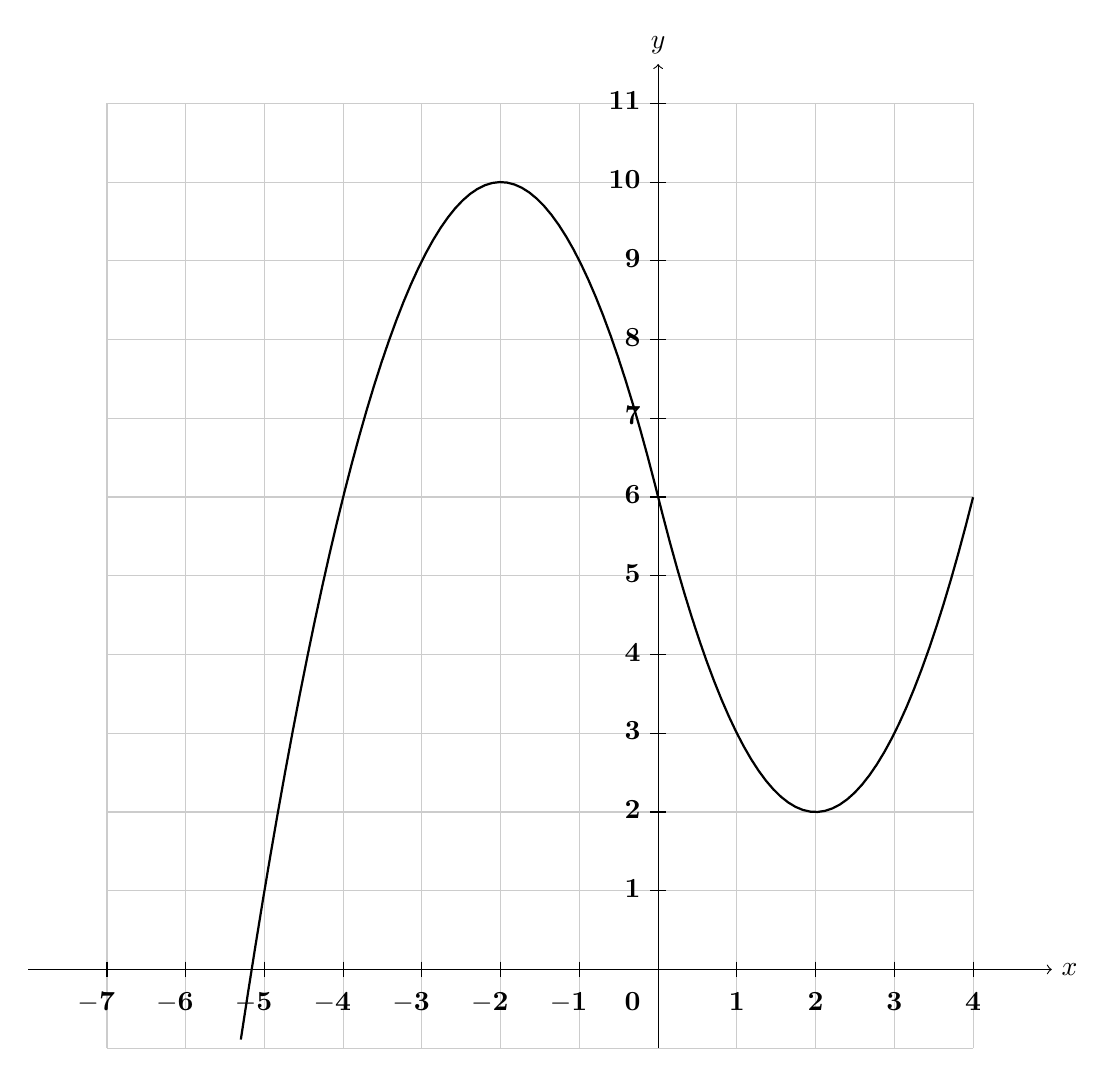
\begin{tikzpicture}
     		\draw[color=gray!40] (-7,-1) grid (4,11);
     		\draw[->] (-8,0) -- (5,0) node[right] {$x$};
     		\draw[->] (0,-1) -- (0,11.5) node[above] {$y$};
     		\foreach \x in {-7,...,-1}{\draw (\x,0.1cm) -- (\x,-0.1cm) node[below] {$\mathbf{\x}\phantom{-}\strut$};}
     		\foreach \x in {1,...,4} {\draw (\x,0.1cm) -- (\x,-0.1cm) node[below] {$\mathbf{\x}\strut$};}
     		\foreach \y in {1,2,...,11}{\draw (0.1cm,\y) -- (-0.1cm,\y) node[left] {$\mathbf{\y}\strut$};}

     		\node[below left=0.1cm] at (-0,0) {$\mathbf{0}\strut$};
     		\draw[domain=-5.3:4,samples=100,color=black,thick] plot[variable=\x] ({\x},{\x^2-4*\x+6});
		\end{tikzpicture}
     		}
\end{document}
